\documentclass[tikz,border=0pt]{standalone}
\usepackage{amsmath}
\usetikzlibrary{arrows.meta,calc,decorations.pathmorphing,shadings}
\definecolor{navy}{HTML}{07162D}
\definecolor{blue}{HTML}{56B4E9}
\definecolor{cyan}{HTML}{8DE7F7}
\definecolor{green}{HTML}{8BCB77}
\definecolor{red}{HTML}{D94C55}
\definecolor{rose}{HTML}{F6A4AC}
\definecolor{gold}{HTML}{F6C453}
\definecolor{mist}{HTML}{EAF5F8}
\begin{document}
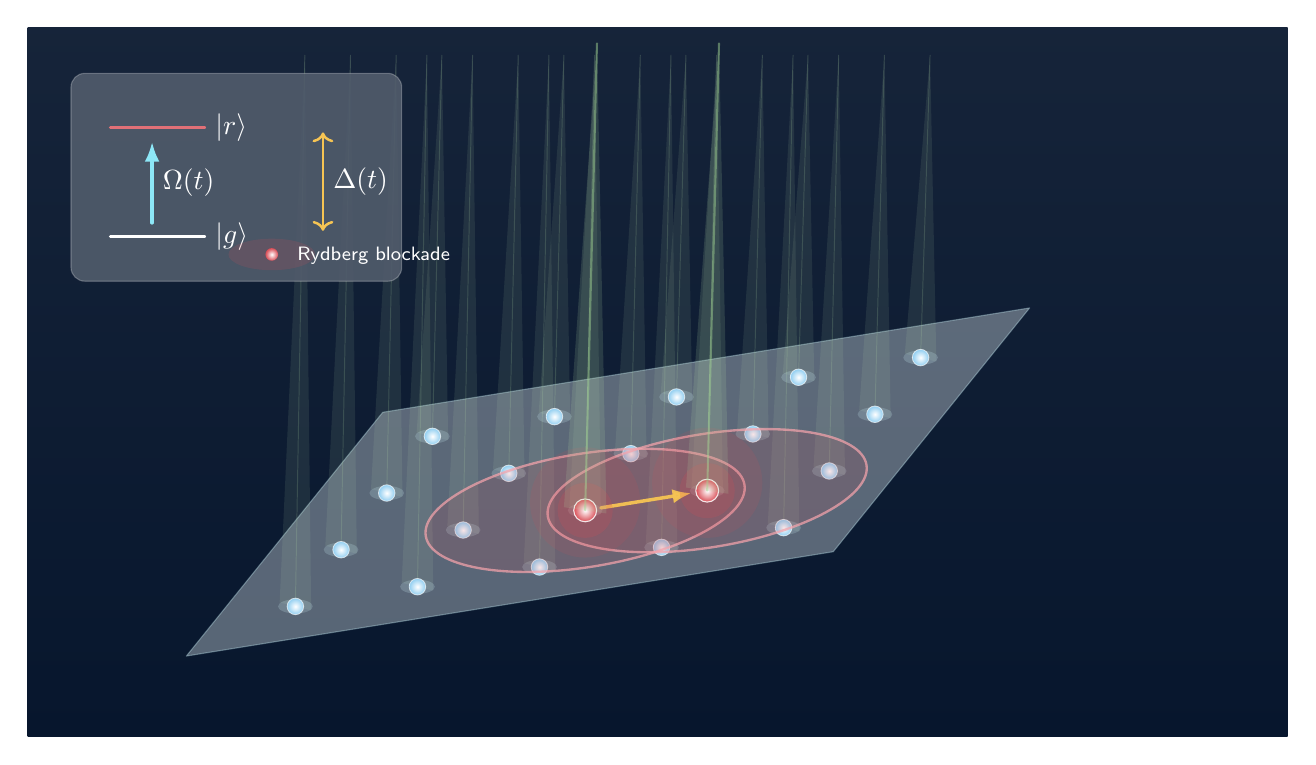
\begin{tikzpicture}[x=1cm,y=1cm,line cap=round,line join=round]
  \path[use as bounding box] (0,0) rectangle (16,9);
  \shade[top color=navy!94,bottom color=navy] (0,0) rectangle (16,9);

  % One projected plane and one affine basis define the complete 5 x 4 array.
  % The tabletop is the lattice footprint expanded by the same margin in lattice
  % coordinates, so its edges are exactly parallel to the atom rows and columns.
  \coordinate (origin) at (3.40,1.65);
  \coordinate (u) at (1.55,.25);
  \coordinate (v) at (.58,.72);
  \fill[blue!10,opacity=.35]
    (2.0155,1.0195) -- (10.2305,2.3445) -- (12.7245,5.4405) -- (4.5095,4.1155) -- cycle;
  \draw[cyan!45,opacity=.35]
    (2.0155,1.0195) -- (10.2305,2.3445) -- (12.7245,5.4405) -- (4.5095,4.1155) -- cycle;

  % Tweezer columns terminate exactly at the affine lattice sites.
  \foreach \j in {0,...,3}{
    \foreach \i in {0,...,4}{
      \pgfmathsetmacro{\xx}{3.40 + 1.55*\i + .58*\j}
      \pgfmathsetmacro{\yy}{1.65 + .25*\i + .72*\j}
      \pgfmathsetmacro{\topx}{\xx + .12}
      \fill[green!55,opacity=.10] (\topx,8.65) -- (\xx-.20,\yy+.05) -- (\xx+.20,\yy-.05) -- cycle;
      \draw[green!65,opacity=.18,line width=.35pt] (\topx,8.65) -- (\xx,\yy);
      \fill[cyan!40,opacity=.20] (\xx,\yy) ellipse (.22 and .09);
      \shade[inner color=white,outer color=blue!65] (\xx,\yy) circle (.105);
      \draw[white,opacity=.65,line width=.3pt] (\xx,\yy) circle (.105);
    }
  }

  % Adjacent sites (2,1) and (3,1) are selected from that same lattice.
  \coordinate (A) at (7.08,2.87);
  \coordinate (B) at (8.63,3.12);
  \fill[red,opacity=.14,rotate around={9.16:(A)}] (A) ellipse (2.05 and .72);
  \fill[red,opacity=.14,rotate around={9.16:(B)}] (B) ellipse (2.05 and .72);
  \draw[rose,opacity=.72,line width=.85pt,rotate around={9.16:(A)}] (A) ellipse (2.05 and .72);
  \draw[rose,opacity=.72,line width=.85pt,rotate around={9.16:(B)}] (B) ellipse (2.05 and .72);
  \fill[red,opacity=.12] ($(A)+(0,0.10)$) circle (.70);
  \fill[red,opacity=.12] ($(B)+(0,0.10)$) circle (.70);
  \draw[-{Latex[length=2.4mm]},gold,line width=1.25pt,opacity=.95] ($(A)+(.20,.032)$) -- ($(B)+(-.20,-.032)$);
  \foreach \p in {A,B}{
    \fill[red,opacity=.20] (\p) circle (.35);
    \shade[inner color=white,outer color=red] (\p) circle (.145);
    \draw[white,opacity=.85,line width=.4pt] (\p) circle (.145);
  }

  % Two stronger excitation beams make the selected pair legible at thumbnail size.
  \fill[green!65,opacity=.16] (7.23,8.8) -- ($(A)+(-.27,.04)$) -- ($(A)+(.27,-.04)$) -- cycle;
  \fill[green!65,opacity=.16] (8.78,8.8) -- ($(B)+(-.27,.04)$) -- ($(B)+(.27,-.04)$) -- cycle;
  \draw[green!80,opacity=.48,line width=.75pt] (7.23,8.8) -- (A);
  \draw[green!80,opacity=.48,line width=.75pt] (8.78,8.8) -- (B);

  % Compact physical legend, patterned after a scientific figure rather than a logo.
  \fill[navy!70,rounded corners=5pt,opacity=.90] (.55,5.78) rectangle (4.75,8.42);
  \draw[white,opacity=.25,rounded corners=5pt] (.55,5.78) rectangle (4.75,8.42);
  \draw[white,line width=1pt] (1.05,6.35) -- (2.25,6.35) node[right,white] {$|g\rangle$};
  \draw[red!80,line width=1pt] (1.05,7.73) -- (2.25,7.73) node[right,white] {$|r\rangle$};
  \draw[-{Latex[length=2.5mm]},cyan,line width=1.2pt] (1.58,6.52) -- (1.58,7.55)
    node[midway,right,white] {$\Omega(t)$};
  \draw[<->,gold,line width=.9pt] (3.75,6.42) -- (3.75,7.67)
    node[midway,right,white] {$\Delta(t)$};
  \fill[red,opacity=.16] (3.10,6.12) ellipse (.55 and .20);
  \shade[inner color=white,outer color=red] (3.10,6.12) circle (.08);
  \node[white,anchor=west,font=\sffamily\scriptsize] at (3.30,6.10) {Rydberg blockade};
\end{tikzpicture}
\end{document}
